\documentclass[a4paper,12]{article}

%\usepackage{times}
\usepackage{fancyhdr}
\usepackage[utf8]{inputenc}
\usepackage{circuitikz}
\usepackage[top=2cm,bottom=2cm,right=2cm,left=2cm]{geometry}
\usepackage{array}
\usepackage{multirow}
\usepackage{hhline}
\usepackage{float}

\pagestyle{fancy}   
\lhead{Digital Electronics}
\rhead{Group Assignment}
\cfoot{\thepage} 
\title{
    \begin{figure}[H]
        \centering
        
\includegraphics{mak_logo.png}
    \end{figure}
    \textbf {COLLEGE OF ENGINEERING, DESIGN, ART AND TECHNOLOGY\\
    DEPARTMENT OF ELECTRICAL AND COMPUTER ENGINEERING\\
    SCHOOL OF ENGINEERING\\
    BACHELOR OF SCIENCE IN ELECTRICAL ENGINEERING\\
    YEAR THREE\\
    ELE3103: APPLIED DIGITAL ELECTRONICS\\
    ASSIGNMENT 1\\
    GROUP \\
}
}
\date{August 2023}
\begin{document}

\maketitle
\begin{center}
    \begin{tabular}{|l|c|c|c|}
        \hline
    \textbf{NAME} & \textbf{COURSE} & \textbf{REG. NO.}\\[10pt] \hline
    Babirye Immaculate & BELE & 21/U/1048 \\[10pt] \hline
    Akirapa Jacky & BELE & 21/U/0637 \\[10pt] \hline
    Nabwire Jovia Namulinda & BELE & 21/U/1352 \\[10pt] \hline
    Mbalire Shawal & BELE & 21/U/0851 \\[10pt] \hline
    Bwire Kennedy & BELE & 21/U/0456 \\[10pt] \hline
    \end{tabular}
\end{center}
\newpage

\section{Question One}

Consider a digital control circuit that controls temperature and pressure in a given system. If the temperature and/or pressure is out of the desired range, the system energizes an indicator light S at the output. A temperature value that is within the desired range is indicated by a HIGH at logic signal T. Pressure is measured in two different points of the system. A pressure value out of range is indicated by two logic signals U and V both of which go HIGH at both points.
\subsection {Design a logic circuit that energizes the indicator light.}
To design a logic circuit that activates the indicator light ($S$), we first establish the truth table to specify the desired behavior. The truth table is as follows:
\begin{center}
    \textbf{Truth Table}
    \vspace{10pt}
    
    \begin{tabular}{|c|c|c||c|}
    \hline
    \textbf{T} & \textbf{U} & \textbf{V} & \textbf{S} \\
    \hline
    0 & 0 & 0 & 1 \\
    0 & 0 & 1 & 1 \\
    0 & 1 & 0 & 1 \\
    0 & 1 & 1 & 1 \\
    1 & 0 & 0 & 0 \\
    1 & 0 & 1 & 0 \\
    1 & 1 & 0 & 0 \\
    1 & 1 & 1 & 1 \\
    \hline
    \end{tabular}
\end{center}

The Karnaugh Map (K-Map) for the output $S$ is as follows:

\begin{center}
    \textbf{K-Map for Output $S$}
    \vspace{10pt}
    
    \begin{tabular}{|c|c|c|}\hline
    S & $\overline{T}$&T  \\\hline
    $\overline{U}\overline{V}$& 1 & 0 \\
    $\overline{U}V$ & 1 & 0 \\
    UV & 1 & 1 \\
    $U\overline{V}$ & 1 & 0 \\
    \hline
    \end{tabular}
\end{center}
\[S=\overline{T}+UV\]
From the K-Map and the given conditions:
\begin{itemize}
    \item  $T$ is HIGH when the temperature is within the desired range.
    \item If both $U$ and $V$ are HIGH, the pressure is out of range.
    \item To energize the light ($S$), we need $T$ to be LOW, and both $U$ and/or $V$ should  be HIGH at the same time.
\end{itemize}

This leads to the following logical expression for $S$:

\[S = not~T ~or~ (U ~and~ V)\]


\begin{center}
\begin{circuitikz}
    \draw
    (4,0) node[and port] (andUV) {}
    (3.5,2) node[not port] (notT) {}
    (6,1) node[or port] (orST) {};
    
    
    \draw (andUV.in 1) -- ++(-1,0) node[left] {U};
    \draw (andUV.in 2) -- ++(-1,0) node[left] {V};
    \draw (notT.in 1) -- ++(-1,0) node[left] {T};
    
    \draw (notT.out) -- (orST.in 1);
    \draw (andUV.out) -- (orST.in 2);
    
    \draw (orST.out) -- ++(1,0) node[right] {S};
\end{circuitikz}
\end{center}


For implementation with a 74LS00N chip, we must change the AND gate to NAND gates. The circuit diagram is as follows:
\begin{center}
    \begin{circuitikz}
        \draw
        (4,0) node[nand port] (andUV) {}
        (6,0) node[nand port] (andUV2) {}
        (6,2) node[nand port] (notT) {}

        (8,2) node[nand port] (ornand1) {}
        (8,0) node[nand port] (ornand2) {}
        (10,1) node[nand port] (ornand3) {};
        
        
        \draw (andUV.in 1) -- ++(-1,0) node[left] {U};
        \draw (andUV.in 2) -- ++(-1,0) node[left] {V};
        \draw (notT.in 1) -- ++(-1,0) node[left] {T};
        \draw (notT.in 2) -- ++(-1,0) node[left] {T};
        
        \draw (andUV.out) -- (andUV2.in 1);
        \draw (andUV.out) -- (andUV2.in 2);
        \draw (andUV2.out) -- (ornand2.in 1);
        \draw (andUV2.out) -- (ornand2.in 2);

        \draw (ornand1.out) -- (ornand3.in 1);
        \draw (ornand2.out) -- (ornand3.in 2);

        \draw (notT.out) -- (ornand1.in 1);
        \draw (notT.out) -- (ornand1.in 2);
        
        \draw (ornand3.out) -- ++(1,0) node[right] {S};
\end{circuitikz}
\end{center}
This circuit, using NAND gates, effectively activates the indicator light $S$ according to the specified conditions for temperature and pressure. It can be implemented with a 74LS00N chip.
\begin{center}
    \begin{circuitikz}
        \draw
        (6,0) node[nand port] (andUV) {}

        (8,1) node[nand port] (ornand3) {};
        
        
        \draw (andUV.in 1) -- ++(-1,0) node[left] {U};
        \draw (andUV.in 2) -- ++(-1,0) node[left] {V};
        \draw (ornand3.in 1) -- ++(-1,0) node[left] {T};
        
        \draw (andUV.out) -- (ornand3.in 2);

        
        \draw (ornand3.out) -- ++(1,0) node[right] {S};
\end{circuitikz}
\end{center}
\[S = \overline{T\overline{UV}}\]


\subsection{Implementing the Circuit with Multisim and 74LS00N Chip}

To demonstrate the practical implementation of the logic circuit, we used Multisim and the 74LS00N quad 2-input NAND gate integrated circuit. The following figures (\ref{fig:1aa} and \ref{fig:1ab}) depict the circuit designed in Multisim. In these figures, we showcase two different scenarios by varying the input values of $U$, $V$, and $T$, with the corresponding output $S$.

\begin{figure}[H]
    \centering
    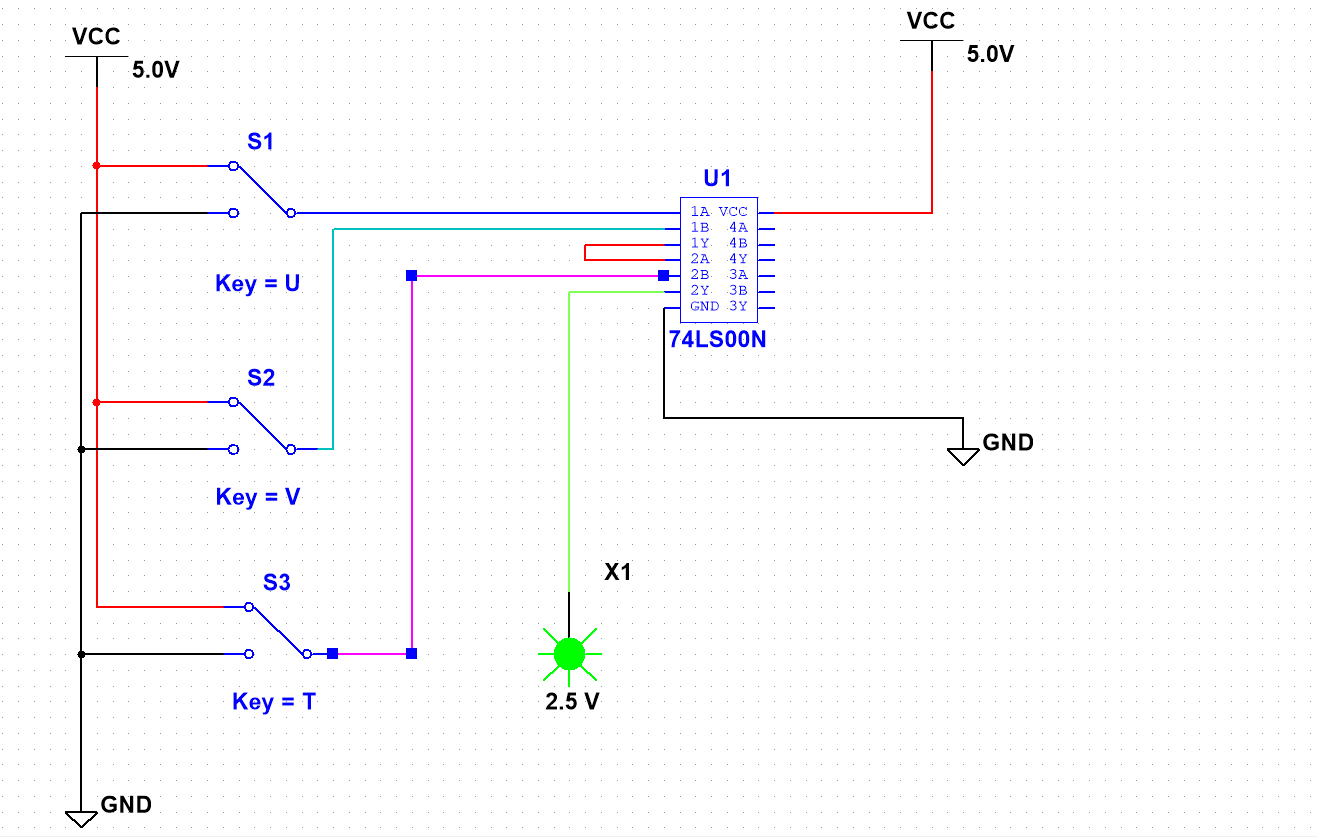
\includegraphics[width=\textwidth]{q1m1.png}
    \caption{Multisim circuit for question 1a, Scenario 1:$ V = 1, U = 1, T = 1$}
    \label{fig:1aa}
\end{figure}
In Figure~\ref{fig:1aa}, we present Scenario 1 where the inputs $U$, $V$, and $T$ have specific values, resulting in an output $S$.  $V=1,U=0,T=1$ and $S=1$. This is also an expected output since the temperature is within the desired range, and the pressure is  out of range.


\begin{figure}[H]
    \centering
    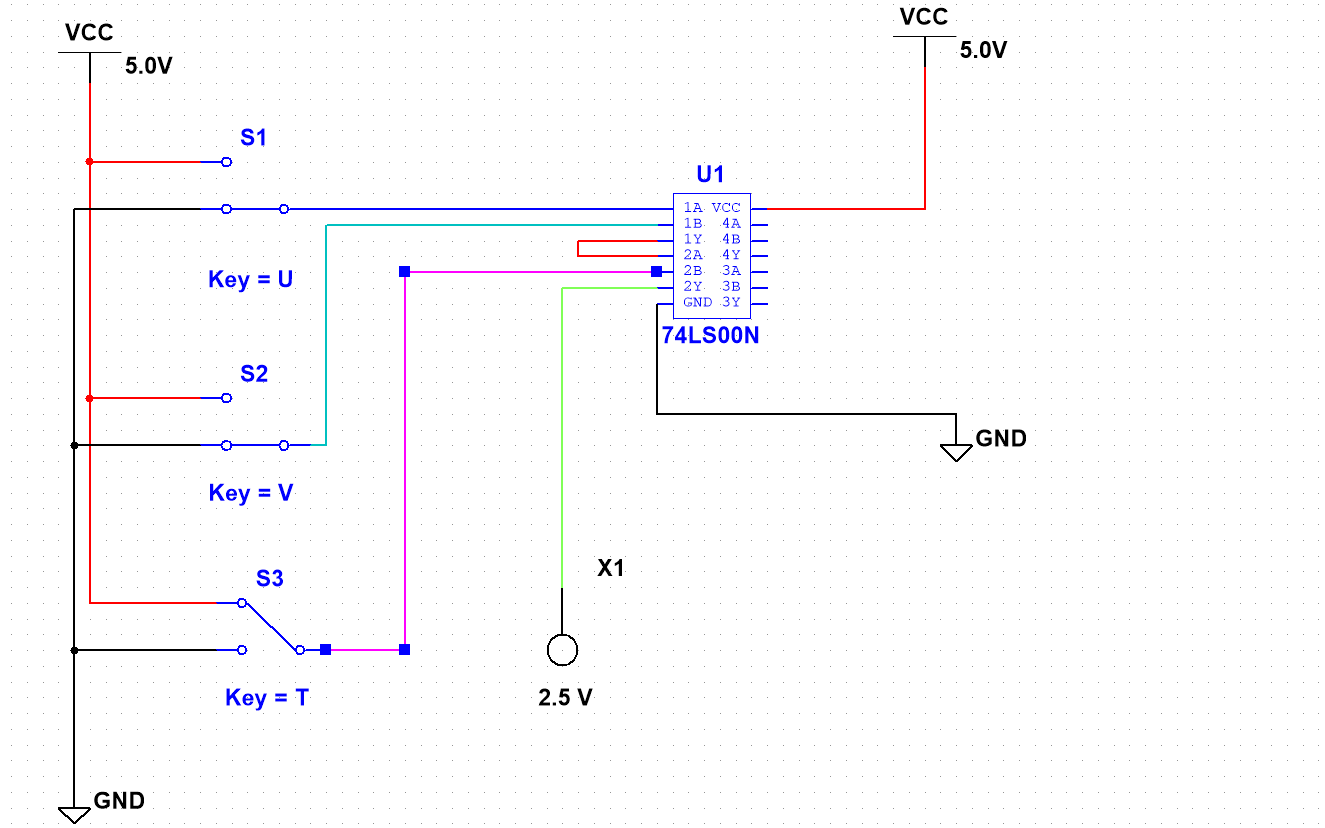
\includegraphics[width=\textwidth]{q1m2.png}
    \caption{Multisim circuit for question 1a, Scenario 2: $V=1,U=0,T=1$}
    \label{fig:1ab}
\end{figure}

In Figure~\ref{fig:1ab}, we illustrate Scenario 2 with a different set of inputs for $U$, $V$, and $T$, leading to a distinct output $S$. $ V = 1, U = 1, T = 1$ and $S = 0$. This is an expected output since the temperature is within the desired range, and the pressure is out of range.
These scenarios demonstrate the practical performance and functionality of the implemented circuit.




\subsection {Use Quartus software to implement the circuit in (a). Show the code, RTL viewer schematic, and timing diagram of the circuit performance.}
The Figures~\ref{fig:1ac} and \ref{fig:1ad} show the circuit implemented in Quartus with U,V,T as high inputs and S as output.

\begin{figure}[H]
    \centering
    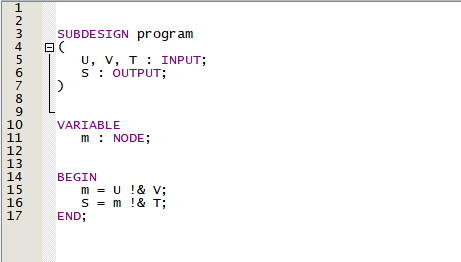
\includegraphics[width=\textwidth]{q1code.png}
    \caption{Quartus Code for question 1a}
    \label{fig:1ad}                                                                                                                               
\end{figure}

Figure~\ref{fig:1ad} showcases the Quartus code used for implementing the logic circuit. The code defines the behavior and connections of the circuit using AHDL and NAND gates.

\begin{figure}[H]
    \centering
    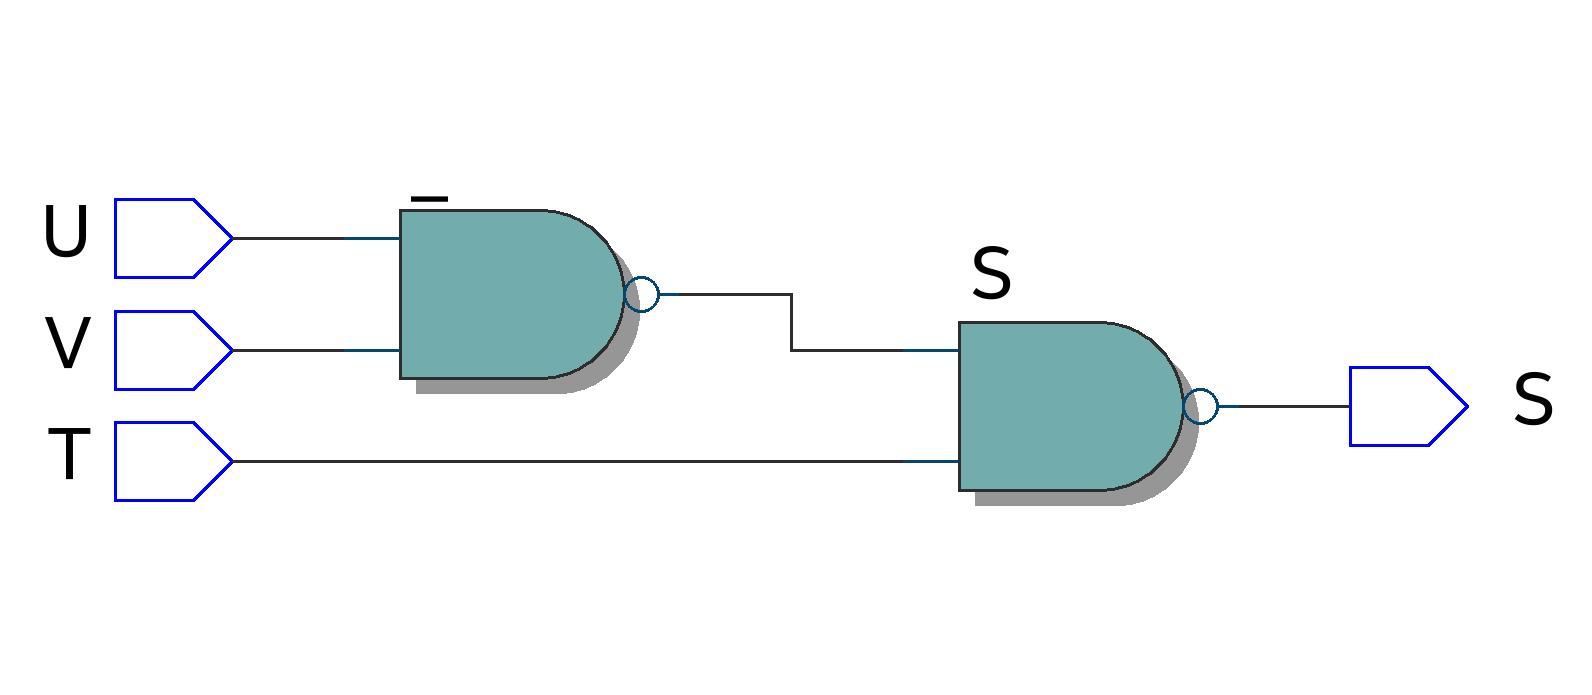
\includegraphics[width=\textwidth]{q1q1.png}
    \caption{Quartus Circuit Schematic for question 1a}
    \label{fig:1ac}
\end{figure}

In Figure~\ref{fig:1ac}, we present the Quartus circuit schematic, which visually represents the implemented logic circuit. The inputs $U$, $V$, and $T$ are set to HIGH, and the output $S$ is displayed.

Furthermore, the RTL viewer schematic in Figure~\ref{fig:1ae} illustrates the doubly implemented NAND gates. They are represented as a NOT gate in this viewer, highlighting the logical structure of the circuit.

\begin{figure}[H]
    \centering
    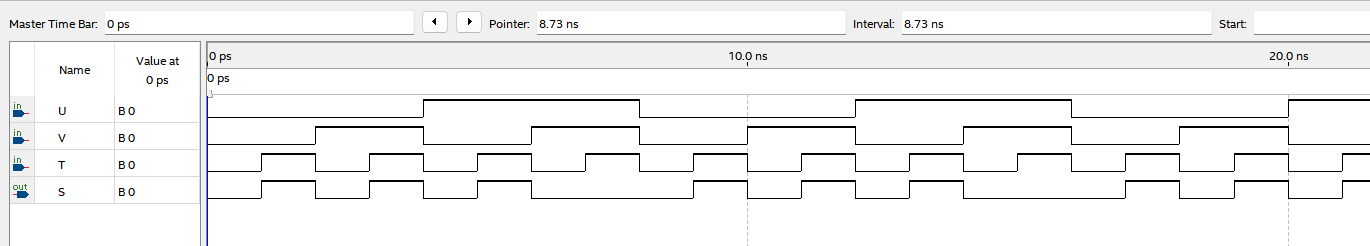
\includegraphics[width=\textwidth]{q1qtiming.png}
    \caption{Quartus Timing Diagram (VWF) for question 1a}
    \label{fig:1ae}
\end{figure}

Figure~\ref{fig:1ae} displays the Quartus Timing Diagram in VWF format, providing insights into the circuit's performance over time. It shows signal waveforms, illustrating how the circuit responds to different input conditions and transitions.


\newpage
\section{Question Two}
Implement a MOD-13 synchronous counter. Ensure that the counter correctly counts through the full cycle. Use a HEX component to display the counting sequence. Add the XLA to view your output. Include only two screenshots in your report. \textbf{Note: I have provided a simple tutorial about using the XLA in a separate document.}
% insert figure here
\begin{figure}[H]
    \centering
    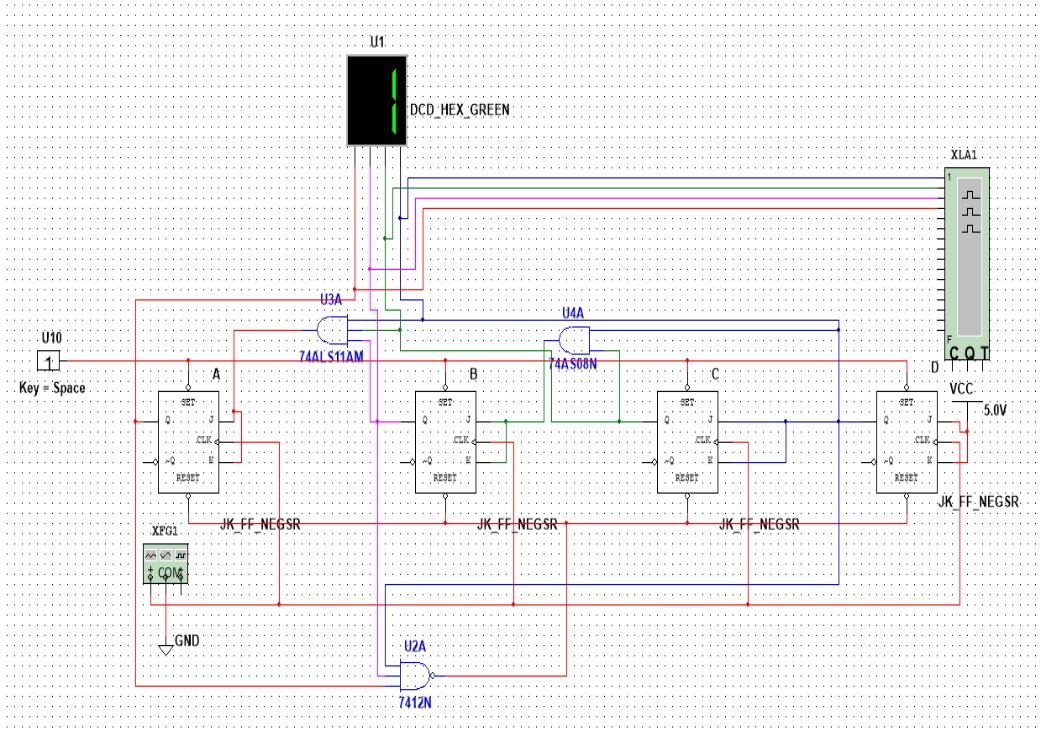
\includegraphics[width=\textwidth]{n21.jpg}
    \caption{Scenario one}
    \label{fig:1ae}
\end{figure}
\begin{figure}[H]
    \centering
    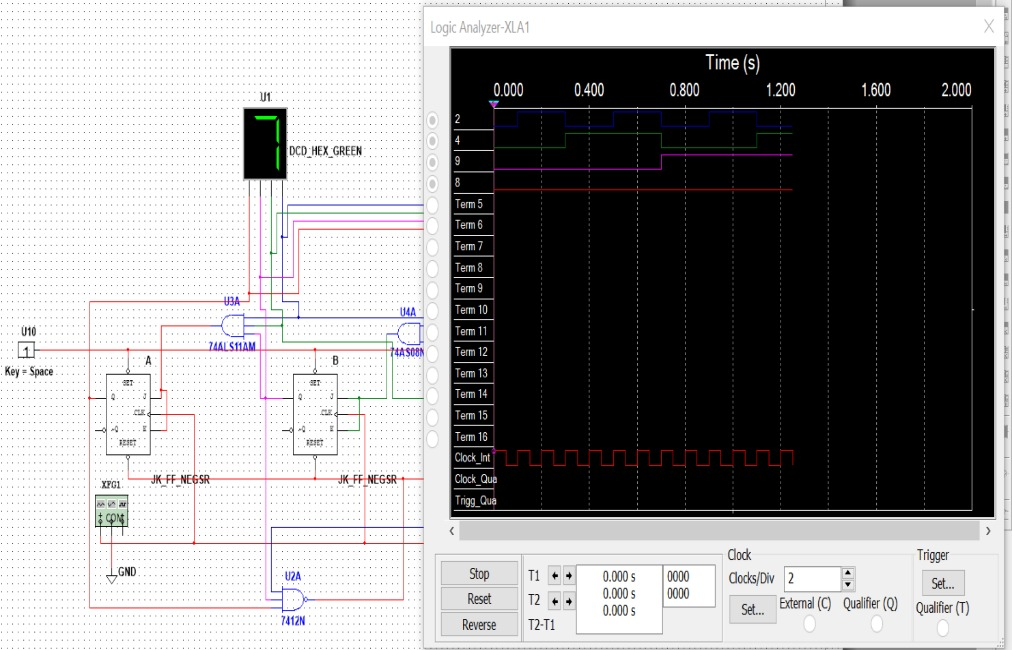
\includegraphics[width=\textwidth]{n22.jpg}
    \caption{Scenario two}
    \label{fig:1ae}
\end{figure}




\newpage
\section{Question Three}
Demonstrate the counting performance of a 74ALS161 IC counter. Use a numeric display (e.g., the SEVEN SEG COM A) to display its count states. Use Multisim.
% insert figure here
\begin{figure}[H]
    \centering
    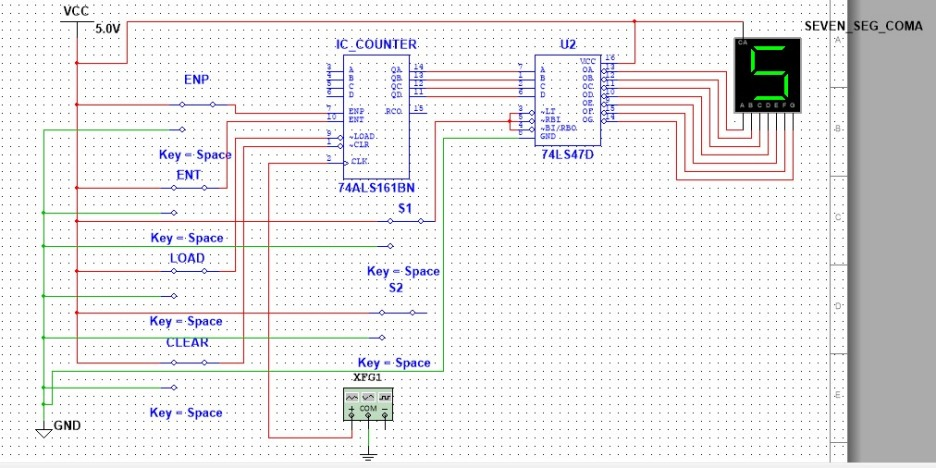
\includegraphics[width=\textwidth]{n31.jpg}
    \caption{Scenario one}
    \label{fig:1ae}
\end{figure}
\begin{figure}[H]
    \centering
    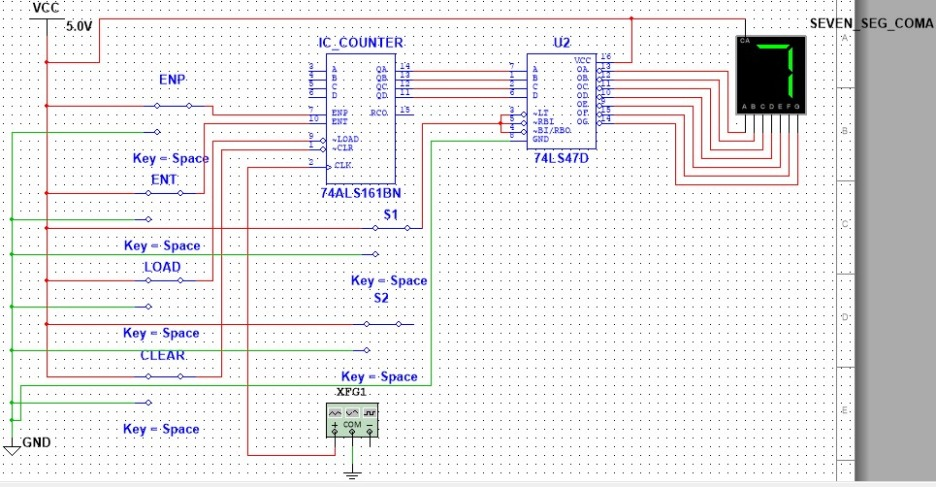
\includegraphics[width=\textwidth]{n32.jpg}
    \caption{Scenario two}
    \label{fig:1ae}
\end{figure}
\begin{figure}[H]
    \centering
    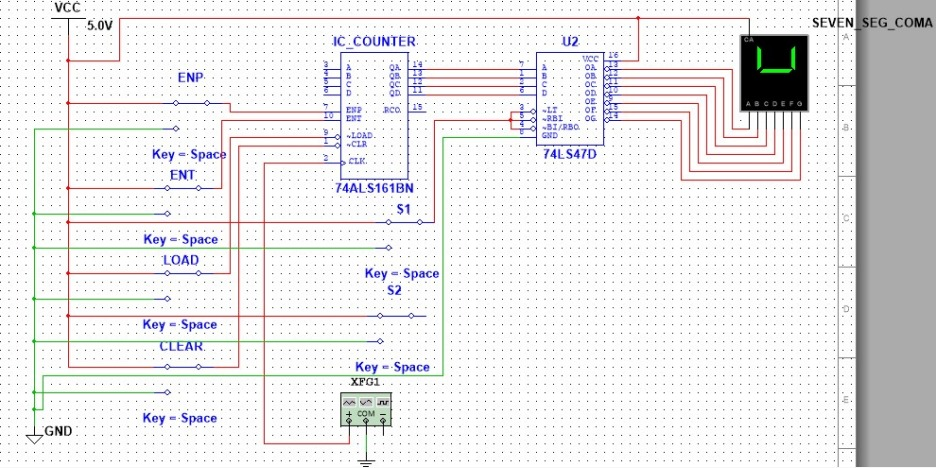
\includegraphics[width=\textwidth]{n33.jpg}
    \caption{Scenario three}
    \label{fig:1ae}
\end{figure}



\newpage
\section{Question Four}
The 7442 BCD-to-Decimal decoder (Fig 9.5) can be used as a 3-line-to-8-line decoder, by using the D input as an ENABLE input (see Problem 9-7). Explain briefly how this arrangement works as an enabled 1-of-8 decoder, and state how the level on D either enables or disables the outputs (show in a truth table). \textbf{Note: This number does not require implementation in Multisim.}\\

\textbf{Solution} 
The 7442 BCD-to-Decimal decoder can be used as a 3-line-to-8-line decoder when the D input serves as an ENABLE input. In this configuration, D will be held active LOW since it is considered as an ENABLE input. When D is set to HIGH (1), it enables the decoder, allowing it to function as a 3-line-to-8-line decoder. 

Since D is considered as an ENABLE input, C, B, and A will be the three inputs, and the outputs will range from 0 to 7 while outputs 8 and 9 will be inactivated since D will be in its INACTIVE state. In this state, the inputs A, B, and C (the 3-line input) are decoded, and one of the eight outputs (Y0 to Y7) is selected based on the binary combination at A, B, and C.

Conversely, when D is LOW (0), it disables the decoder. In this condition, all of the outputs (Y0 to Y7) are rendered inactive. This effectively disconnects the A, B, and C inputs from the decoder, resulting in all outputs remaining at an inactive state.

\textbf{Truth Table:}

Here is a truth table illustrating how the level on D either enables or disables the outputs of the 7442 decoder:


\begin{center}
    \begin{tabular}{|c|c|c|c|c|c|}
    \hline
    \textbf{D} & \textbf{C} & \textbf{B} & \textbf{A} & \textbf{Output} \\
    \hline
    0 & 0 & 0 & 0 & 0 \\
    0 & 0 & 0 & 1 & 1 \\
    0 & 0 & 1 & 0 & 2 \\
    0 & 0 & 1 & 1 & 3 \\
    0 & 1 & 0 & 0 & 4 \\
    0 & 1 & 0 & 1 & 5 \\
    0 & 1 & 1 & 0 & 6 \\
    0 & 1 & 1 & 1 & 7 \\
    1 & 0 & 0 & 0 & None \\
    1 & 0 & 0 & 1 & None \\
    1 & 0 & 1 & 0 & None \\
    1 & 0 & 1 & 1 & None \\
    1 & 1 & 0 & 0 & None \\
    1 & 1 & 0 & 1 & None \\
    1 & 1 & 1 & 0 & None \\
    1 & 1 & 1 & 1 & None \\
    \hline
    \end{tabular}
    \end{center}


\end{document}